% version 1.00	Auteur Mathieu Médici

Le référentiel Livraison contient l'ensemble des livrables de \nomEquipe{}.

\clearpage

\begin{figure}[ht]
         \begin{center}
         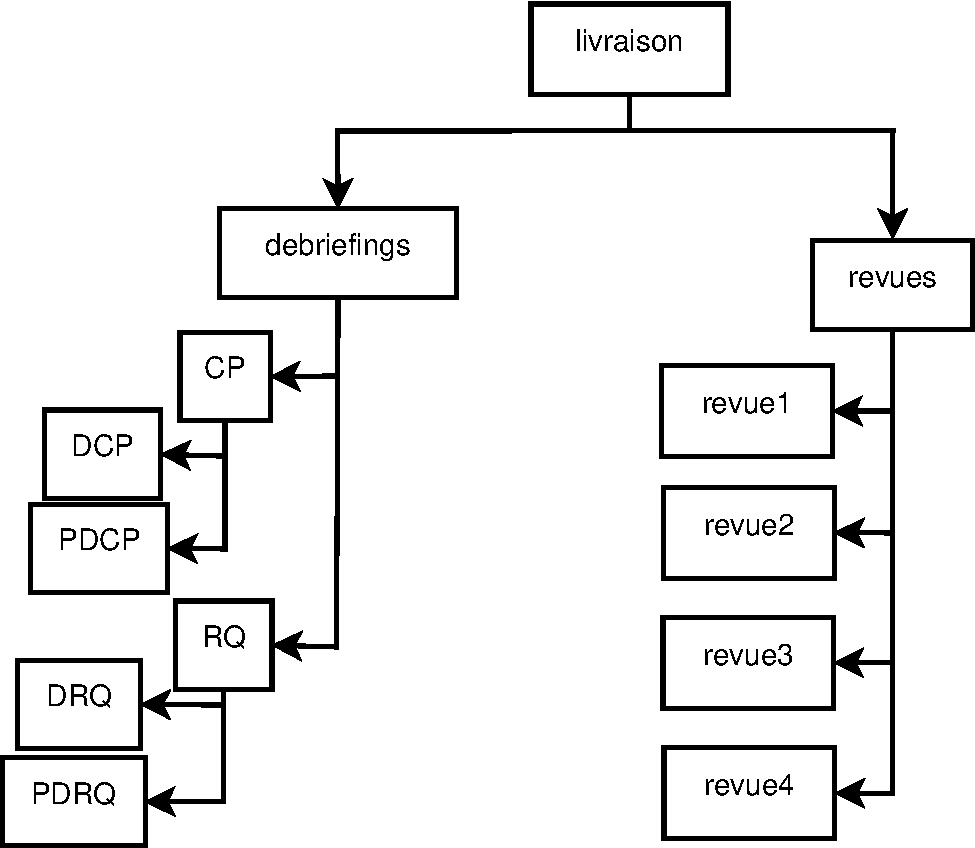
\includegraphics[scale=0.5]{images/arboLivraison}
         \end{center}
         \caption{Référentiel Livraison}
 \end{figure}

%\section{Précisions}


%Le répertoire \textbf{livraisons complémentaires} contient les documents livrés au Client
%en dehors des livraisons officielles des lots. Il se trouve dans le \textbf{FTP}.
%Par exemple, si le Client veut prendre connaissance de notre \planQualite{}, 
%il sera placé dans ce répertoire. 
%Ainsi, ce répertoire permettra le traçage de tout ce qui a été envoyé au client en dehors des livraisons.


%~ Le répertoire \textbf{SP}, placé dans le répertoire \textbf{lots}
%~ correspond au support de présentation dans le cas où il y a une présentation orale
%~ de la part de \nomPIC{} pour le Client.

%Pour le cas où une présentation orale est demandée par le Client, 
%le support de présentation sera placé dans le répertoire \textbf{SP}.
